\documentclass[UTF8, fontset=macnew, a4paper, 12pt]{ctexart}

\usepackage{geometry}
\geometry{top=2.3cm, bottom=2.3cm, left=2.4cm, right=2.4cm}
\usepackage{amsmath, amssymb}
\usepackage{booktabs}
\usepackage{graphicx}
\usepackage{caption}
\usepackage{xcolor}
\usepackage{float}
\usepackage{enumitem}
\usepackage{fancyhdr}
\usepackage[hidelinks]{hyperref}

\graphicspath{{../output/figures/}}
\captionsetup{font=small, labelfont=bf, labelsep=quad}
\setlist{itemsep=2pt, parsep=0pt, topsep=3pt}

\ctexset{
  section/format = \raggedright\zihao{4}\bfseries,
  section/name   = {},
  section/number = \chinese{section}、,
  subsection/format = \raggedright\zihao{5}\bfseries,
  subsection/number = \chinese{subsection}、,
}
\renewcommand{\thesection}{\chinese{section}}
\setcounter{secnumdepth}{2}

\pagestyle{fancy}
\fancyhf{}
\fancyhead[L]{\small 小人口 Lee-Carter 模型之估計與區間推論}
\fancyhead[R]{\small 進度報告（簡版）}
\fancyfoot[C]{\small \thepage}
\renewcommand{\headrulewidth}{0.4pt}

\newcommand{\edag}{e_0^{\dagger}}
\newcommand{\LCe}{\mathrm{LC}e^{\dagger}}

\begin{document}

\begin{center}
{\zihao{3}\bfseries 小人口 Lee-Carter 模型之估計與區間推論}\\[3pt]
{\zihao{5} —— 進度報告（簡版）}\\[10pt]
{\zihao{5} （學生姓名）\quad 指導教授：余清祥\,教授}\\[3pt]
{\zihao{5} 國立政治大學統計學系\qquad 中華民國 115 年 9 月 21 日}
\end{center}

\vspace{4pt}
\begin{center}
\begin{minipage}{0.93\textwidth}\small
\textbf{本文說明}\quad 本簡版摘錄詳細版的研究問題、關鍵數據與結論，
供快速瀏覽之用；各項實驗的設計、判讀邏輯、圖表與完整書目請參閱
《進度報告》（詳細版，共 32 頁）。文中括號內的節號即為詳細版的對應位置。
\end{minipage}
\end{center}

\vspace{8pt}

\section{研究問題}

我國 368 個鄉鎮市區中，217 個（59\%）的單一性別人數在兩萬以下。
此等規模下 Lee-Carter（以下簡稱 LC）模型的年齡參數會出現\textbf{有方向的
偏誤}（Wang et al. 2018；余清祥等 2021）。本文提出三個依序遞進的問題：

\begin{enumerate}[leftmargin=*]
  \item Rabbi and Mazzuco（2021）在國家級資料上成立的優勢，改換資料與
        配適期後是否仍成立？
  \item 小樣本下 LC 模型失效的機制是\textbf{變異數增大}還是\textbf{偏誤}？
        兩者的補救方式完全不同。
  \item 把懲罰項直接加在年齡參數 $\boldsymbol{\beta}$ 上是否可行？
        LASSO、Ridge、Elastic Net 應如何取捨？
\end{enumerate}

\textbf{符號}：$\boldsymbol{\beta}\in\mathbb{R}^{A}$、
$\boldsymbol{\kappa}\in\mathbb{R}^{T}$ 為向量，$\beta_x$、$\kappa_t$ 為其
分量；識別條件為 $\mathbf{1}_A^{\!\top}\boldsymbol{\beta}=1$、
$\mathbf{1}_T^{\!\top}\boldsymbol{\kappa}=0$。
資料為臺灣五齡組 1970$\sim$2024 年，主分析為女性 2001$\sim$2024 年
（$A=22$、$T=24$）。

\section{問題一：復刻的結論與其界限}

\textbf{成立的部分}（詳細版 \S 伍之一）：LASSO 修勻的配適誤差
（MAE 0.0413）確實小於一維與二維 $L_2$ 樣條（0.0538、0.0759）；
$\edag$ 調整亦使 $\kappa_t$ 更接近線性（離線性殘差標準差由 LC 的 0.960
降至 0.726）。

\textbf{不成立的部分}（\S 伍之二）：

\begin{enumerate}[leftmargin=*]
  \item \textbf{優勢僅限於近期短配適期。} 擴充為「性別 $\times$ 起始年」
        12 格面板後，$\LCe$ 僅在 2001、1991 年起算的 5 格勝出，
        其餘 7 格全由 Lee-Miller 奪冠，1981、1971 年起算的長配適期
        \textbf{無一例外}。全人口 1970$\sim$2024 年時 $\edag$ 調整甚至使
        $\kappa_t$ \textbf{更不線性}（1.824 對 LC 的 0.848）。
  \item \textbf{預測區間不是更窄而是最寬。} $\LCe$ 的 2050 年 $e_0$
        區間寬度 3.977 為六種方法之最。原因是「$\kappa_t$ 更線性」與
        「$\kappa_t$ 變異更小」並不等價。
  \item \textbf{涵蓋率的優勢以寬度換得}，且六種方法的實證涵蓋率
        全落在 0.2$\sim$0.6，離名目 0.8 甚遠。
\end{enumerate}

另有三項方法論問題（\S 伍之三）：原文比較 $e_0$ 與 $\edag$ 相關係數的
論證因 LC 秩為一而\textbf{必然近乎完美相關}；$\edag$ 對 $\kappa$ 為
\textbf{單峰而非單調}，對齊原則上可能有兩個解；該文選修勻參數的準則
（對觀測值的誤差）\textbf{必然選到不修勻}。

\section{問題二：失效的機制是偏誤}

以蒙地卡羅模擬建立已知真值的環境（重複 100 次，$\lambda$ 以
$\lambda_{\max}$ 正規化）。\textbf{判準}：若只是變異數問題，各指標應環繞
真值對稱散布；若有偏誤，指標的中位數本身會系統性偏離。

\begin{table}[H]
\centering
\caption{暴露數對估計的影響（漂移項真值 $-0.3678$）}
\small
\begin{tabular}{rcccc}
\toprule
$N$ & 零死亡格／528 & $\alpha_x$ 平均偏誤 & $\beta_x$ 相關中位數 & 漂移項中位數\\
\midrule
10,000    & 214.0 & $\mathbf{+0.439}$ & $-0.240$ & $-0.110$\\
50,000    & 89.2  & $+0.033$ & $-0.045$ & $-0.065$\\
200,000   & 21.7  & $-0.051$ & $+0.564$ & $-0.216$\\
1,000,000 & 0.3   & $-0.021$ & $+0.823$ & $-0.340$\\
\bottomrule
\end{tabular}
\end{table}

\textbf{結果與「純變異數」假說不吻合}：$\alpha_x$ 偏誤在 $N=1$ 萬時達
$+0.439$、方向一致為正；漂移項中位數在所有 $N$ 下\textbf{一律偏向零}、
從未高估。兩者皆為系統性方向偏移（\S 陸之一）。

四項延伸結論：

\begin{itemize}[leftmargin=*]
  \item \textbf{區間同時「太寬」且「涵蓋不足」}（\S 陸之五）。$N=5$ 萬時
        現行作法寬 5.401（不可約下限 1.743）、涵蓋率卻僅 0.38。
        \textbf{小樣本的問題是位置而非寬度，加寬區間無濟於事}。
  \item \textbf{修勻確實使區間過窄，且 $N$ 越大越嚴重}（涵蓋率
        $0.66\to0.45\to0.38$）。此即 Basellini et al.（2023）提出但
        未量化的疑慮。
  \item \textbf{配適期長度比人口規模更關鍵}（\S 陸之六）。$T=10$ 年時即使
        $N=10^6$，$\hat\beta$ 與真值的相關僅 0.120；$T=55$ 年時 $N$ 僅
        兩萬也達 0.746。以 0.8 為門檻，$T{=}55$ 需 $N\ge5$ 萬、$T{=}40$ 需
        20 萬、$T{=}30$ 需 100 萬，而 $T\le20$ 年時\textbf{任何人口規模
        都達不到}。
  \item \textbf{兩步校正}（\S 陸之七）：以卜瓦松最大概似取代奇異值分解可
        消除漂移項衰減（$N=5$ 萬時偏誤由 $+0.336$ 降至 $-0.010$）；
        再以拔靴法去除 $\hat\sigma$ 的估計雜訊。合併後在 $N\ge10^6$ 時
        區間寬度 1.721 幾乎追平不可約下限 1.726，涵蓋率 0.83 對名目 0.80。
\end{itemize}

\section{問題三：懲罰式估計}

\textbf{關鍵前提}（\S 柒之二）：在識別條件 $\mathbf{1}_A^{\!\top}
\boldsymbol{\beta}=1$ 之下，
\[
\textstyle\sum_x|\beta_x|=\sum_x\beta_x+2\sum_x\max(-\beta_x,0)
=1+2\sum_x\max(-\beta_x,0),
\]
亦即 $L_1$ 懲罰\textbf{只罰負部}。當 $\hat\beta_x$ 全為正（大人口必然如此），
懲罰項恆為常數、\textbf{估計值完全不動}——實測 $\lambda$ 由 0 加到 $10^6$，
變動量始終在機器精度（$10^{-15}$）之內。

本文因此取收縮目標 $\boldsymbol{\beta}_0=\mathbf{1}_A/A$，其意義為
\textbf{「各年齡以相同速度改善」的虛無假設}，LASSO 的稀疏性即回答
「哪些年齡組顯著偏離平均」。

\begin{table}[H]
\centering
\caption{三種懲罰的比較（$N=20$ 萬，重複 100 次，各取其最適 $\lambda$）}
\small
\begin{tabular}{lcccc}
\toprule
方法 & 最適 $\lambda/\lambda_{\max}$ & 偏誤$^2$ & 變異數 & MSE\\
\midrule
未懲罰 & 0 & 0.00024 & 0.01691 & 0.01698\\
LASSO & 0.030 & 0.00147 & 0.00560 & 0.00702\\
Elastic Net & 0.030 & 0.00158 & 0.00534 & 0.00687\\
Ridge & 0.003 & 0.00270 & 0.00311 & \textbf{0.00578}\\
\bottomrule
\end{tabular}
\end{table}

\begin{itemize}[leftmargin=*]
  \item \textbf{在小樣本效益極大}：$N=5$ 萬時最適
        $\lambda/\lambda_{\max}=0.20$，$\beta$ 的均方誤差由 0.1606 降至
        0.0101（\textbf{降低 94\%}），變異數降 99\%。
  \item \textbf{懲罰縮小的是變異數的常數項而非收斂階數}：$N=2$ 萬時
        變異數 4.391 對 0.022（差 197 倍），但 log-log 斜率 $-1.77$
        對 $-1.27$。
  \item \textbf{固定比例的懲罰在 $N\ge3\times10^5$ 後反而有害}
        （偏誤不隨 $N$ 消失），故 $\lambda$ 必須隨人口規模調整
        （最適比例由 0.20 降至 0.03）。
  \item \textbf{純看均方誤差，Ridge 優於 LASSO}。真值 $\beta_x$ 無一恰等於
        $1/A$，\textbf{稀疏性並非正確的先驗}。另試 MCP、自適應 LASSO、
        鬆弛 LASSO 三種變體，\textbf{亦無一勝過單純的 Ridge}（\S 柒之九）。
  \item LASSO 的價值在\textbf{可解釋性}：在均方誤差與可解釋性之間的權衡
        約為 20\%。目的為估計精確度則用 Ridge／Elastic Net，
        目的為辨識關鍵年齡組則用 LASSO。
\end{itemize}

\begin{figure}[H]
\centering
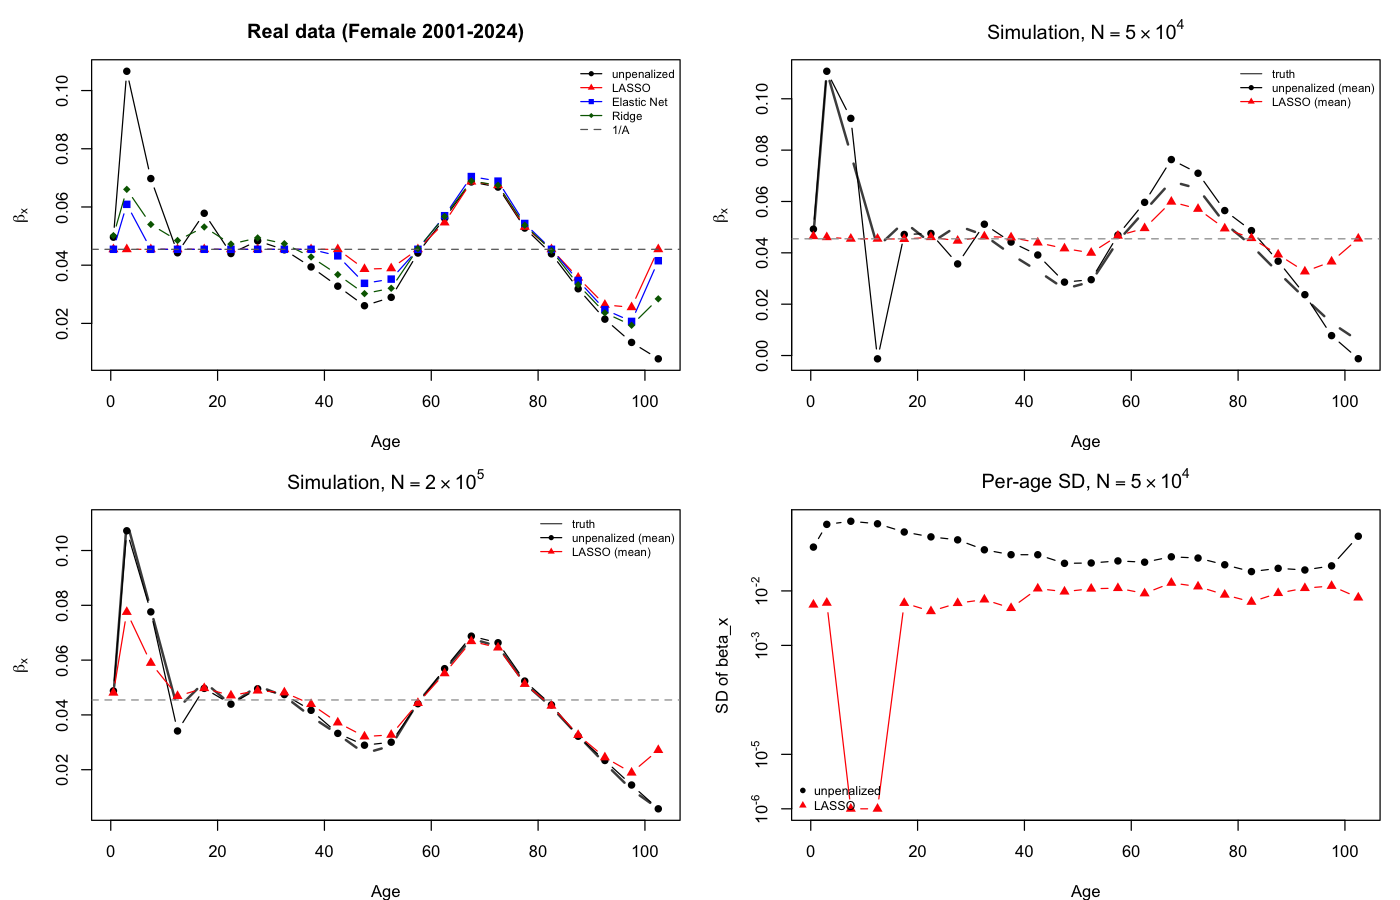
\includegraphics[width=0.86\textwidth]{figA_beta_by_age.png}
\caption{懲罰前後 $\beta_x$ 的逐年齡比較（詳細版附錄A）。
左上為實際資料，右上與左下為模擬的平均估計值（含真值），右下為逐年齡標準差。}
\end{figure}

附錄的逐年齡比較顯示，\textbf{1--4 歲的未懲罰估計值最大（0.1066）卻被完全
併入 $1/A$}——LASSO 的軟閾值為 $\lambda w_x/W_x$，其中
$W_x=\sum_t\hat\mu_{xt}\kappa_t^2$ 為該年齡的資訊量，幼兒死亡數極少使
$W_x$ 很小，故估計值雖大卻不精確，反受最重的懲罰。
\textbf{懲罰強弱取決於資訊量而非係數大小}；存活下來的是 45--54 歲與
60--99 歲，與人口學認知相符。

\section{研究限制與後續工作}

\textbf{限制}：五齡組本身即是強力的變異數縮減器，所得門檻是
「五齡組之下」的門檻；模擬真值取自 LC 配適，隱含「模型正確」的假設，
所得應視為下界；留出期涵蓋 COVID-19。

\textbf{後續工作}：

\begin{enumerate}[leftmargin=*]
  \item 補跑 2001$\sim$2019 年作為 COVID-19 的對照。
  \item 以單齡組資料重新檢驗，分離「五齡組使 $\edag$ 的離散近似誤差偏大」
        與「臺灣死亡轉型較快」兩個競爭解釋。
  \item 量化初始值選擇在準確度與穩健度之間的權衡——這是目前殘餘涵蓋
        誤差的主要來源。
  \item \textbf{假設母體的敏感度分析}：以
        $\boldsymbol{\beta}^{\text{true}}(\delta)=(1-\delta)
        \hat{\boldsymbol{\beta}}^{\text{全國}}+\delta\mathbf{v}$ 做受控偏離，
        比較高齡改善較快、幼年改善較快、中年反轉三個方向，
        檢驗本文各項門檻是否維持。
  \item \textbf{壓力測試}：$\kappa_t$ 跳躍（結構性衝擊）、$\beta_x$ 緩慢
        旋轉（違反 LC 核心假設）、負二項過度離散、人口降至 5,000，
        以界定「在何種條件下本方法不應使用」。
  \item 懲罰強度的自動選取，以及自適應權重與收斂理論的補強。
\end{enumerate}

\vspace{8pt}
\hrule
\vspace{6pt}
\noindent\small
完整的實驗設計、判讀邏輯、全部圖表與書目，請參閱《進度報告》詳細版。
程式碼與可重現的輸出：\texttt{github.com/rickyllin/-20260908}。

\end{document}
